\documentclass[11pt]{article}

\usepackage[margin=1in]{geometry}
\usepackage{amsmath, amssymb, amsthm}
\usepackage{booktabs}
\usepackage{graphicx}
\usepackage{hyperref}
\usepackage{microtype}
\usepackage{xcolor}

\hypersetup{
  colorlinks=true,
  linkcolor=blue!55!black,
  citecolor=blue!55!black,
  urlcolor=blue!55!black
}

\graphicspath{{../outputs/}}

\title{\textbf{Typos on a Page}\\
\large Three Small Probability Models for Isolated and Bursty Errors}
\author{Applied probability note}
\date{\today}

\newcommand{\Prb}{\mathbb{P}}
\newcommand{\E}{\mathbb{E}}
\newcommand{\ind}{\mathbf{1}}

\begin{document}

\maketitle

\begin{abstract}
This note develops three elementary stochastic models for page-level typos.
The first model treats pages as independent Bernoulli trials. The second
introduces a latent Markov state for a fresh or tired typist, producing bursts
through persistent unobserved fatigue. The third treats typos themselves as a
discrete-time self-exciting point process, in the style of a Hawkes process.
The aim is not to solve a high-stakes inference problem, but to show how a
small change in probabilistic structure changes the qualitative behavior of a
sequence of errors. Cumulative crossing probabilities are useful, but
inter-typo gap distributions are the clearest diagnostic of genuine
self-excitation.
\end{abstract}

\section{Setup}

Suppose a document is read page by page. Let
\[
X_k =
\begin{cases}
1, & \text{if page } k \text{ has at least one typo},\\
0, & \text{otherwise}.
\end{cases}
\]
The basic object of interest is the page sequence
\[
X_1, X_2, \ldots, X_n.
\]
For a threshold \(q \in (0,1)\), define the crossover page
\[
n^\star(q) =
\min\left\{n : \Prb\left(\sum_{k=1}^n X_k \ge 1\right) > q\right\}.
\]
This quantity answers a simple question: how many pages must be read before
the chance of seeing at least one typo exceeds a chosen probability level?

The more interesting question is not only when the first typo appears, but
whether typos arrive as isolated accidents or in clusters. The following three
models separate those ideas.

\section{Model I: Independent Page Typos}

The independent baseline assigns each page its own typo probability. In the
original experiment this probability increases linearly with page number:
\[
p_k = 0.01 + \alpha k.
\]
Assuming independence across pages,
\[
\Prb(X_k=1) = p_k,
\qquad
X_1,\ldots,X_n \text{ independent}.
\]
Then the probability of no typo in the first \(n\) pages is
\[
\Prb(X_1=0,\ldots,X_n=0)
= \prod_{k=1}^n (1-p_k),
\]
so
\[
\Prb\left(\sum_{k=1}^n X_k \ge 1\right)
= 1 - \prod_{k=1}^n (1-p_k).
\]

This model is a clean baseline: it captures changing page-level risk but has no
mechanism for clustering. Conditional on the probabilities \(p_k\), a typo on
one page carries no information about nearby pages.

\begin{figure}[htbp]
  \centering
  
\includegraphics[width=0.92\linewidth]{crossover_curves_with_fits.png}
  \caption{Independent-page model. The crossover page \(n^\star\) decreases as
  the slope \(\alpha\) increases. Power-law curves provide a compact empirical
  description of the threshold curves, although the lowest threshold is the
  least well described by this fit.}
  \label{fig:independent-fit}
\end{figure}

\section{Model II: Hidden Markov Tired Typist}

The second model introduces a latent state
\[
S_k \in \{F,T\},
\]
where \(F\) means fresh and \(T\) means tired. Typo probability depends on the
hidden state:
\[
\Prb(X_k=1\mid S_k=F) = p_F,
\qquad
\Prb(X_k=1\mid S_k=T) = p_T,
\]
with \(p_T > p_F\).

The state evolves as a two-state Markov chain:
\[
\Prb(S_{k+1}=T\mid S_k=F)=b,
\qquad
\Prb(S_{k+1}=T\mid S_k=T)=a.
\]
Using state order \((F,T)\), the transition matrix is
\[
P =
\begin{pmatrix}
1-b & b\\
1-a & a
\end{pmatrix}.
\]
The parameter \(a\) is the persistence of tiredness. The expected length of a
tired run is
\[
\E[\text{tired run}] = \frac{1}{1-a}.
\]
Thus \(a=0.92\) corresponds to an expected tired run of \(12.5\) pages, while
\(a=0.98\) corresponds to \(50\) pages.

\subsection{Survival Recursion}

The scalar product from the independent model is replaced by a two-entry
survival vector:
\[
v_k =
\left[
\Prb(X_1=\cdots=X_k=0, S_k=F),
\Prb(X_1=\cdots=X_k=0, S_k=T)
\right].
\]
At each page, the vector is multiplied by the no-typo emission probabilities
\[
d = (1-p_F,\, 1-p_T),
\]
and then propagated through the transition matrix. In code, this is the
recursion
\[
v \leftarrow v \odot d,
\qquad
\Prb(X_1=\cdots=X_k=0)=v_F+v_T,
\qquad
v \leftarrow vP.
\]
The cumulative probability of at least one typo is again one minus the
survival probability.

\begin{figure}[htbp]
  \centering
  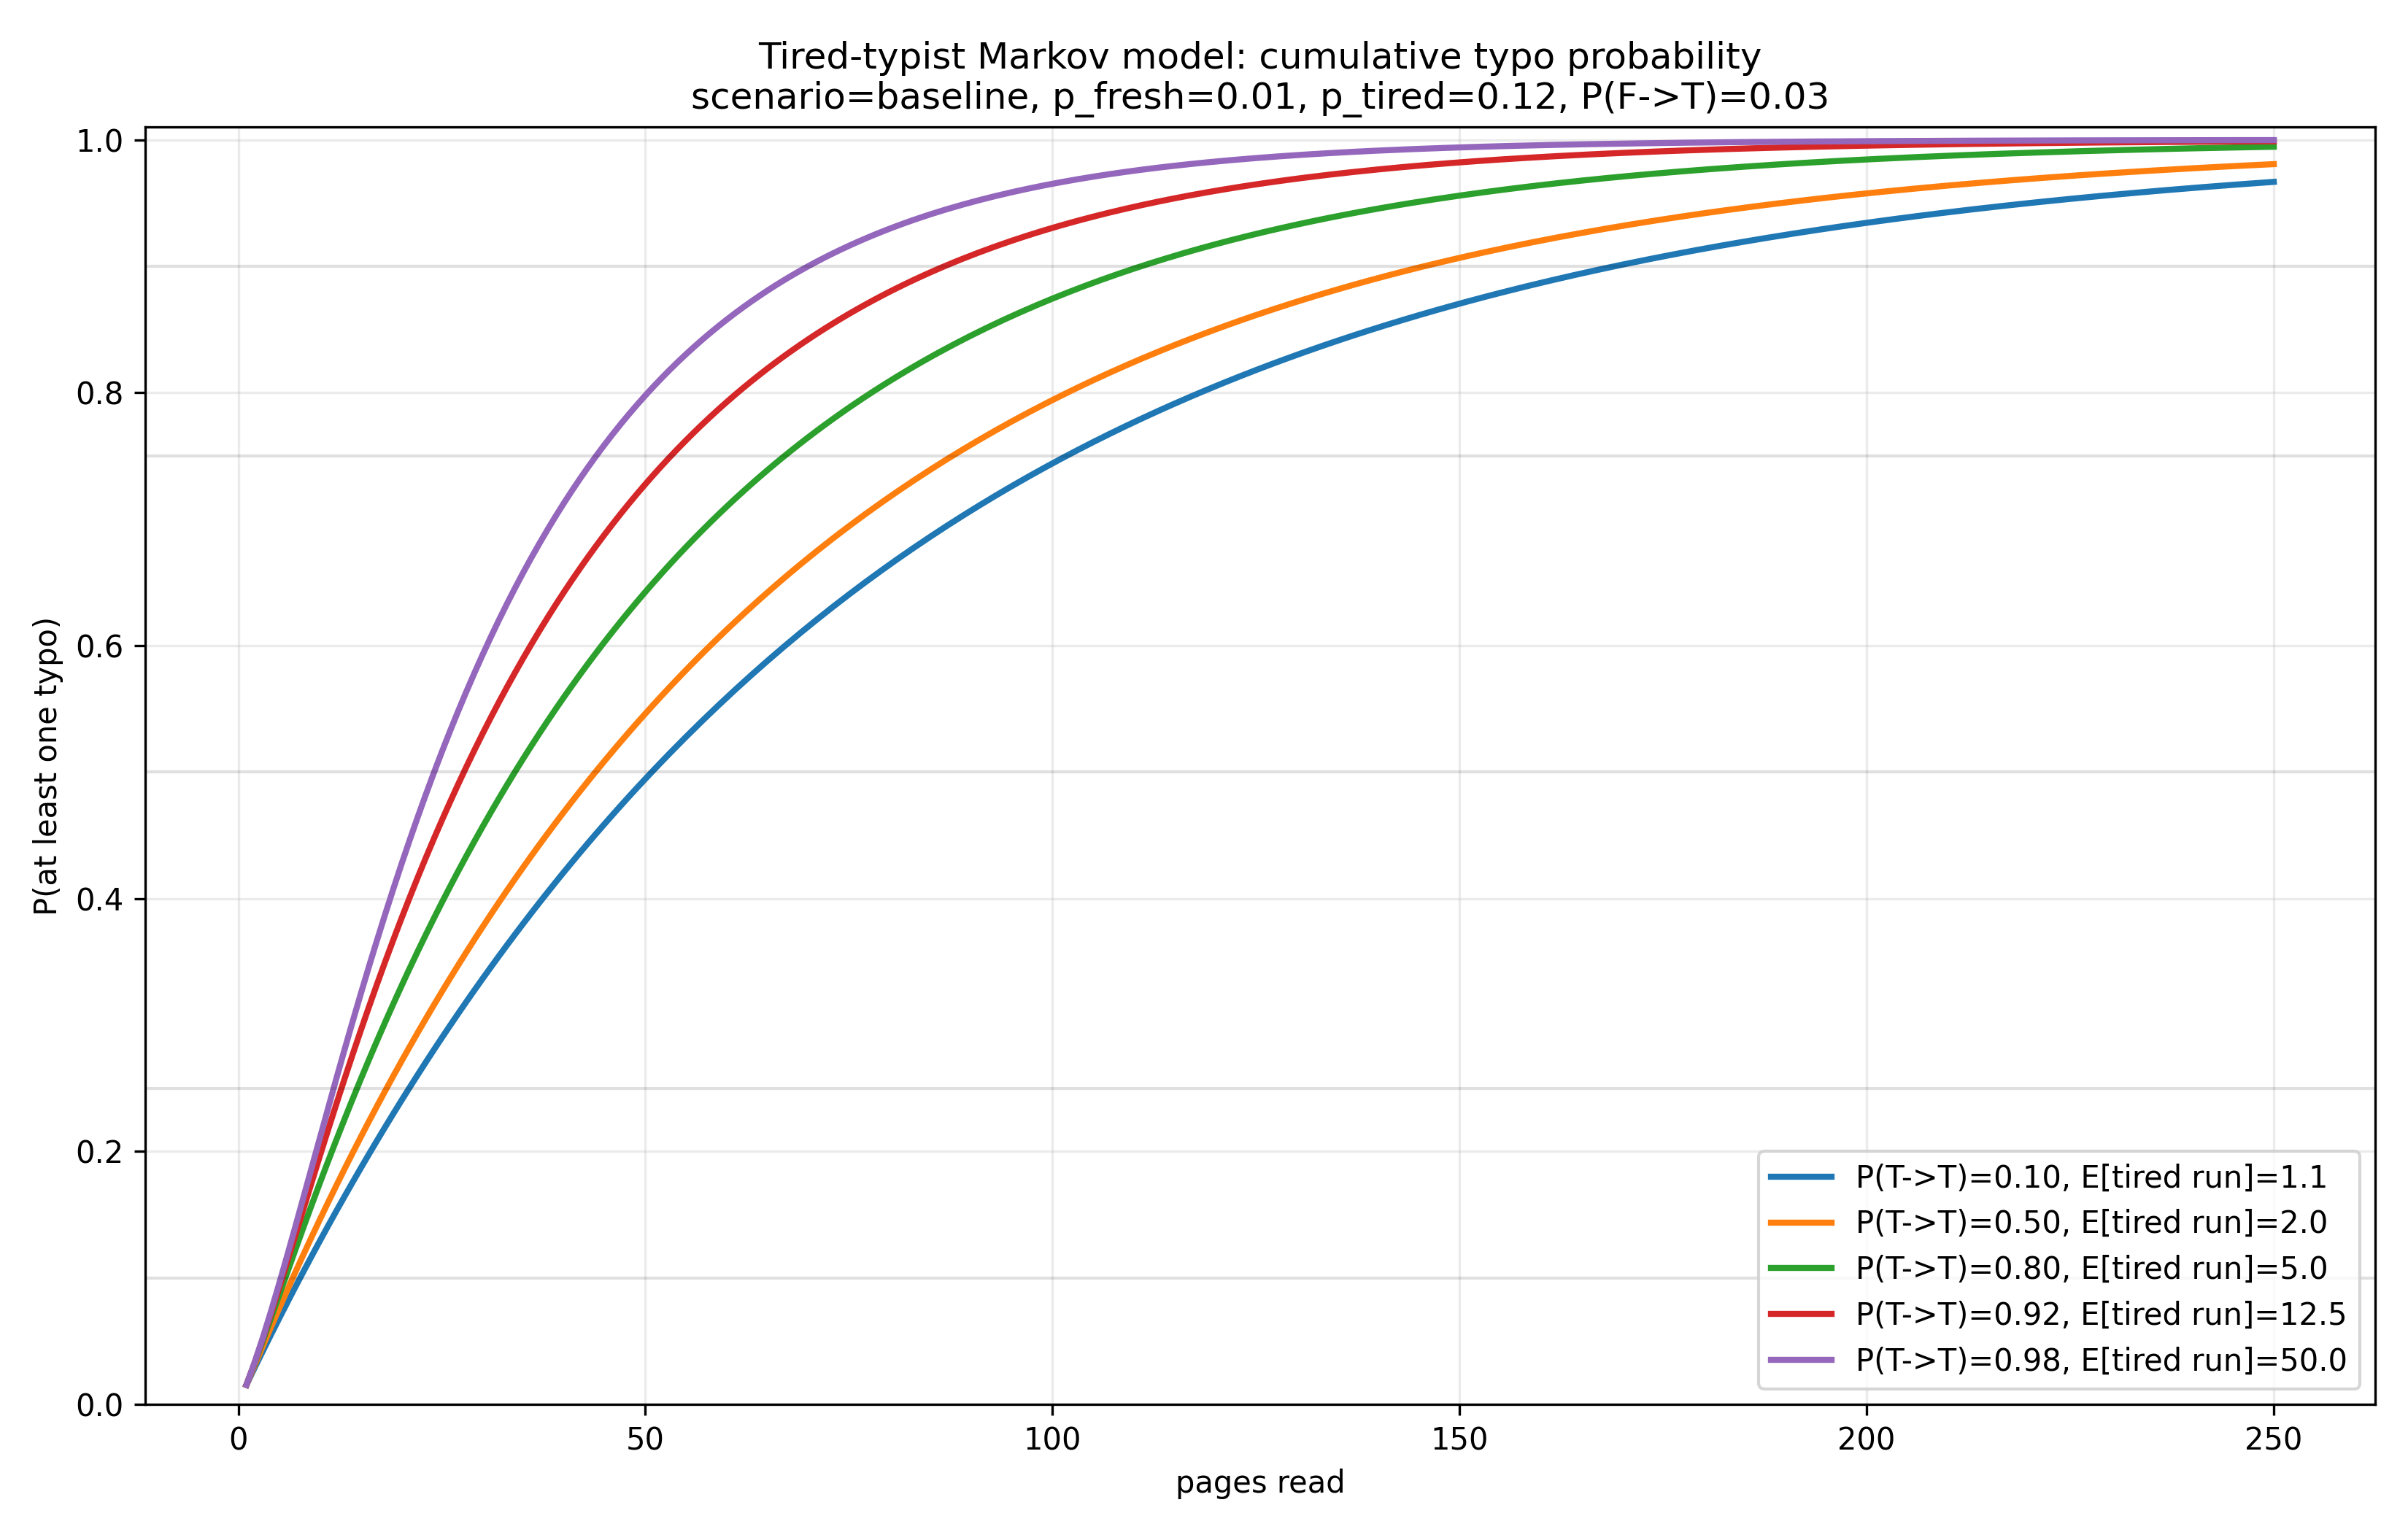
\includegraphics[width=0.92\linewidth]{markovian_probability_curves_baseline.png}
  \caption{Hidden Markov tired-typist model. Larger tired-state persistence
  raises the cumulative probability of seeing at least one typo. The label
  \(E[\text{tired run}]\) shows the expected duration of a tired spell.}
  \label{fig:markov-probability}
\end{figure}

\begin{figure}[htbp]
  \centering
  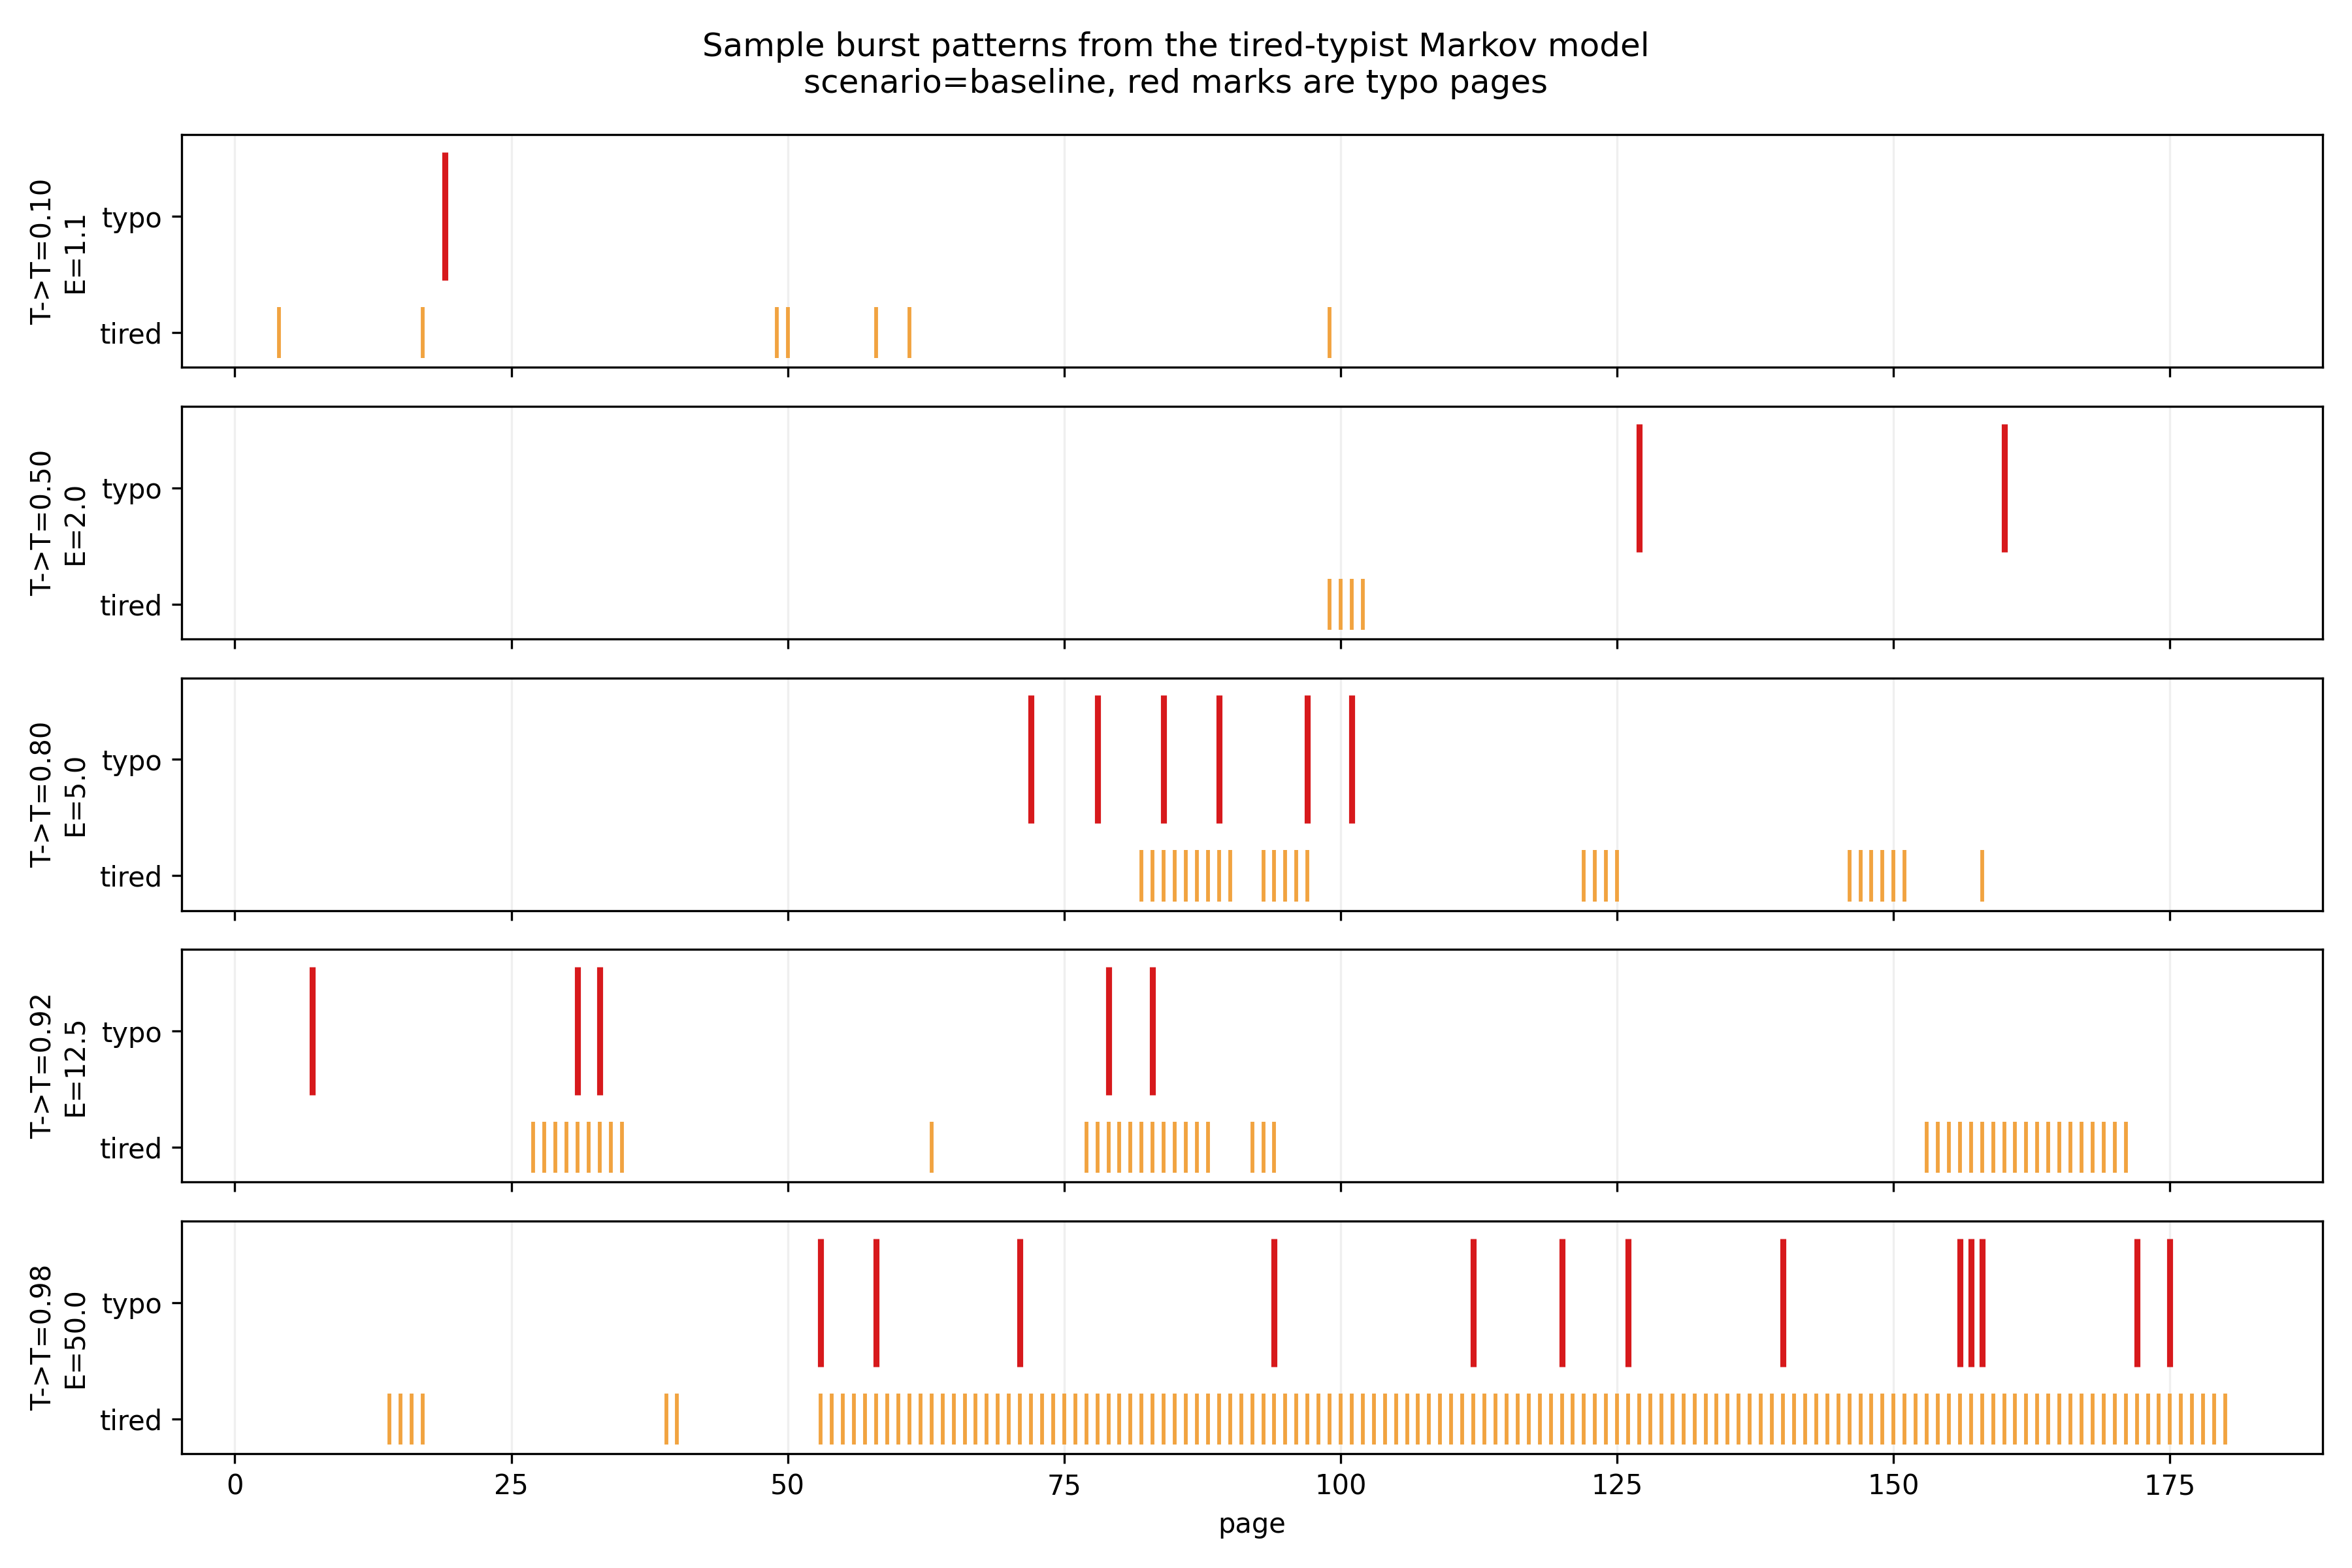
\includegraphics[width=0.95\linewidth]{markovian_sample_bursts_baseline.png}
  \caption{Sample paths from the hidden Markov model. Orange marks indicate
  pages where the latent typist state is tired; red marks indicate typo pages.
  Blank regions are fresh pages with no typo. As tiredness persistence
  increases, long tired stretches become visible and typos cluster within
  them.}
  \label{fig:markov-bursts}
\end{figure}

\section{Model III: Hawkes-Like Self-Exciting Typos}

The third model removes the latent state and makes the observed typo process
self-exciting. A typo increases the near-future typo intensity directly.

Let \(\lambda_k\) denote the page-time typo intensity. The discrete Hawkes-like
recursion used here is
\[
\lambda_k = \mu + E_k,
\]
where
\[
E_k = \delta E_{k-1} + \eta X_{k-1}.
\]
Here \(\mu\) is the baseline intensity, \(\eta\) is the jump in future
intensity caused by a typo, and \(\delta\) is the persistence of excitation.
Intensity is converted to a Bernoulli probability by
\[
\Prb(X_k=1\mid \mathcal{H}_{k-1})
= 1-\exp(-\lambda_k),
\]
where \(\mathcal{H}_{k-1}\) is the history through page \(k-1\).

One useful diagnostic is the approximate branching ratio
\[
R = \frac{\eta\delta}{1-\delta}.
\]
Values below one are the natural stable regime. The three scenarios used in
the experiments are shown in Table~\ref{tab:hawkes-scenarios}.

\begin{table}[htbp]
  \centering
  \begin{tabular}{lccc}
    \toprule
    Scenario & \(\mu\) & \(\eta\) & \(\delta\) \\
    \midrule
    Mild & 0.012 & 0.10 & 0.45 \\
    Baseline & 0.014 & 0.22 & 0.58 \\
    Volatile & 0.010 & 0.35 & 0.72 \\
    \bottomrule
  \end{tabular}
  \caption{Hawkes-like page-time scenarios. The volatile case is deliberately
  close to the high-excitation regime, producing visibly stronger clusters.}
  \label{tab:hawkes-scenarios}
\end{table}

\begin{figure}[htbp]
  \centering
  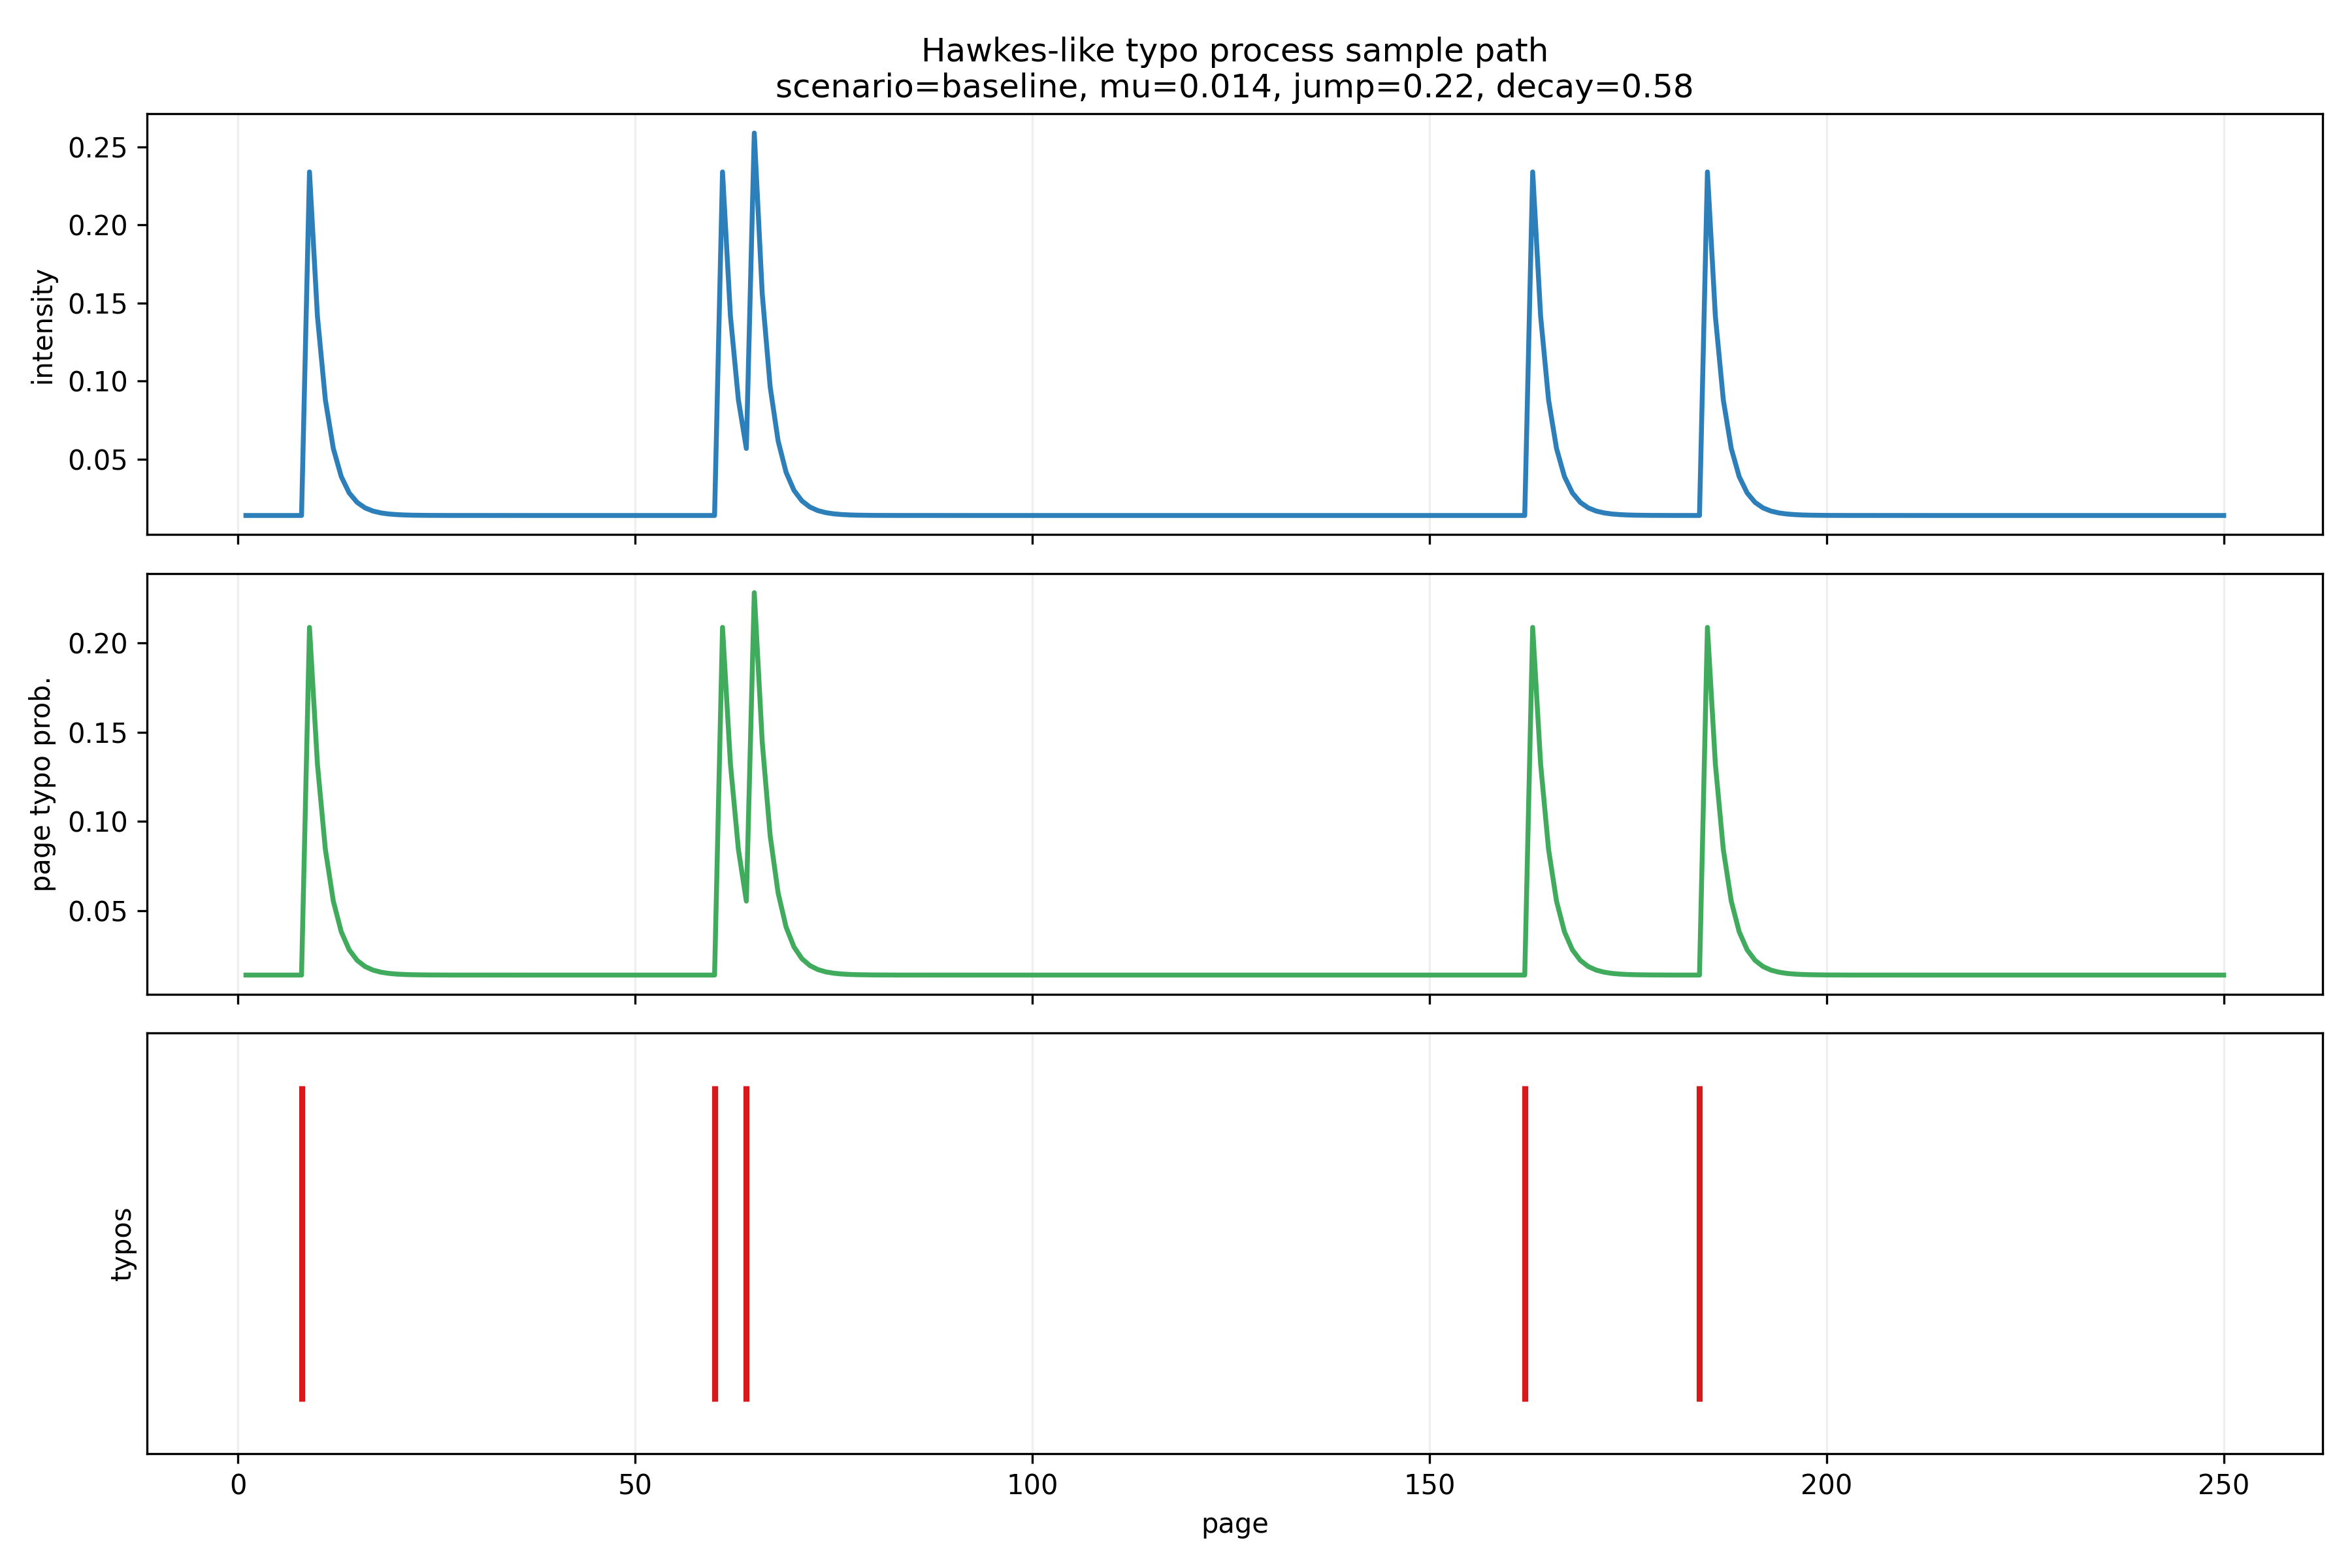
\includegraphics[width=0.95\linewidth]{hawkes_sample_path_baseline.png}
  \caption{A baseline Hawkes-like sample path. A typo event raises the
  intensity and therefore the next few page-level typo probabilities. In quiet
  periods, excitation decays geometrically.}
  \label{fig:hawkes-sample}
\end{figure}

\section{Comparing the Three Models}

For the comparison plots, the independent model is calibrated to match the
long-run average page typo probability of the baseline hidden Markov model.
This makes it a fair non-bursty reference point. The models compared are:
\begin{enumerate}
  \item independent calibrated Bernoulli pages;
  \item hidden Markov tired typist;
  \item baseline Hawkes-like self-exciting process.
\end{enumerate}

\subsection{Cumulative Probability}

Cumulative probability curves answer when the first typo is likely to appear.
They are useful, but they do not fully reveal the dependence structure. A model
can have a high chance of at least one typo without being very bursty.

\begin{figure}[htbp]
  \centering
  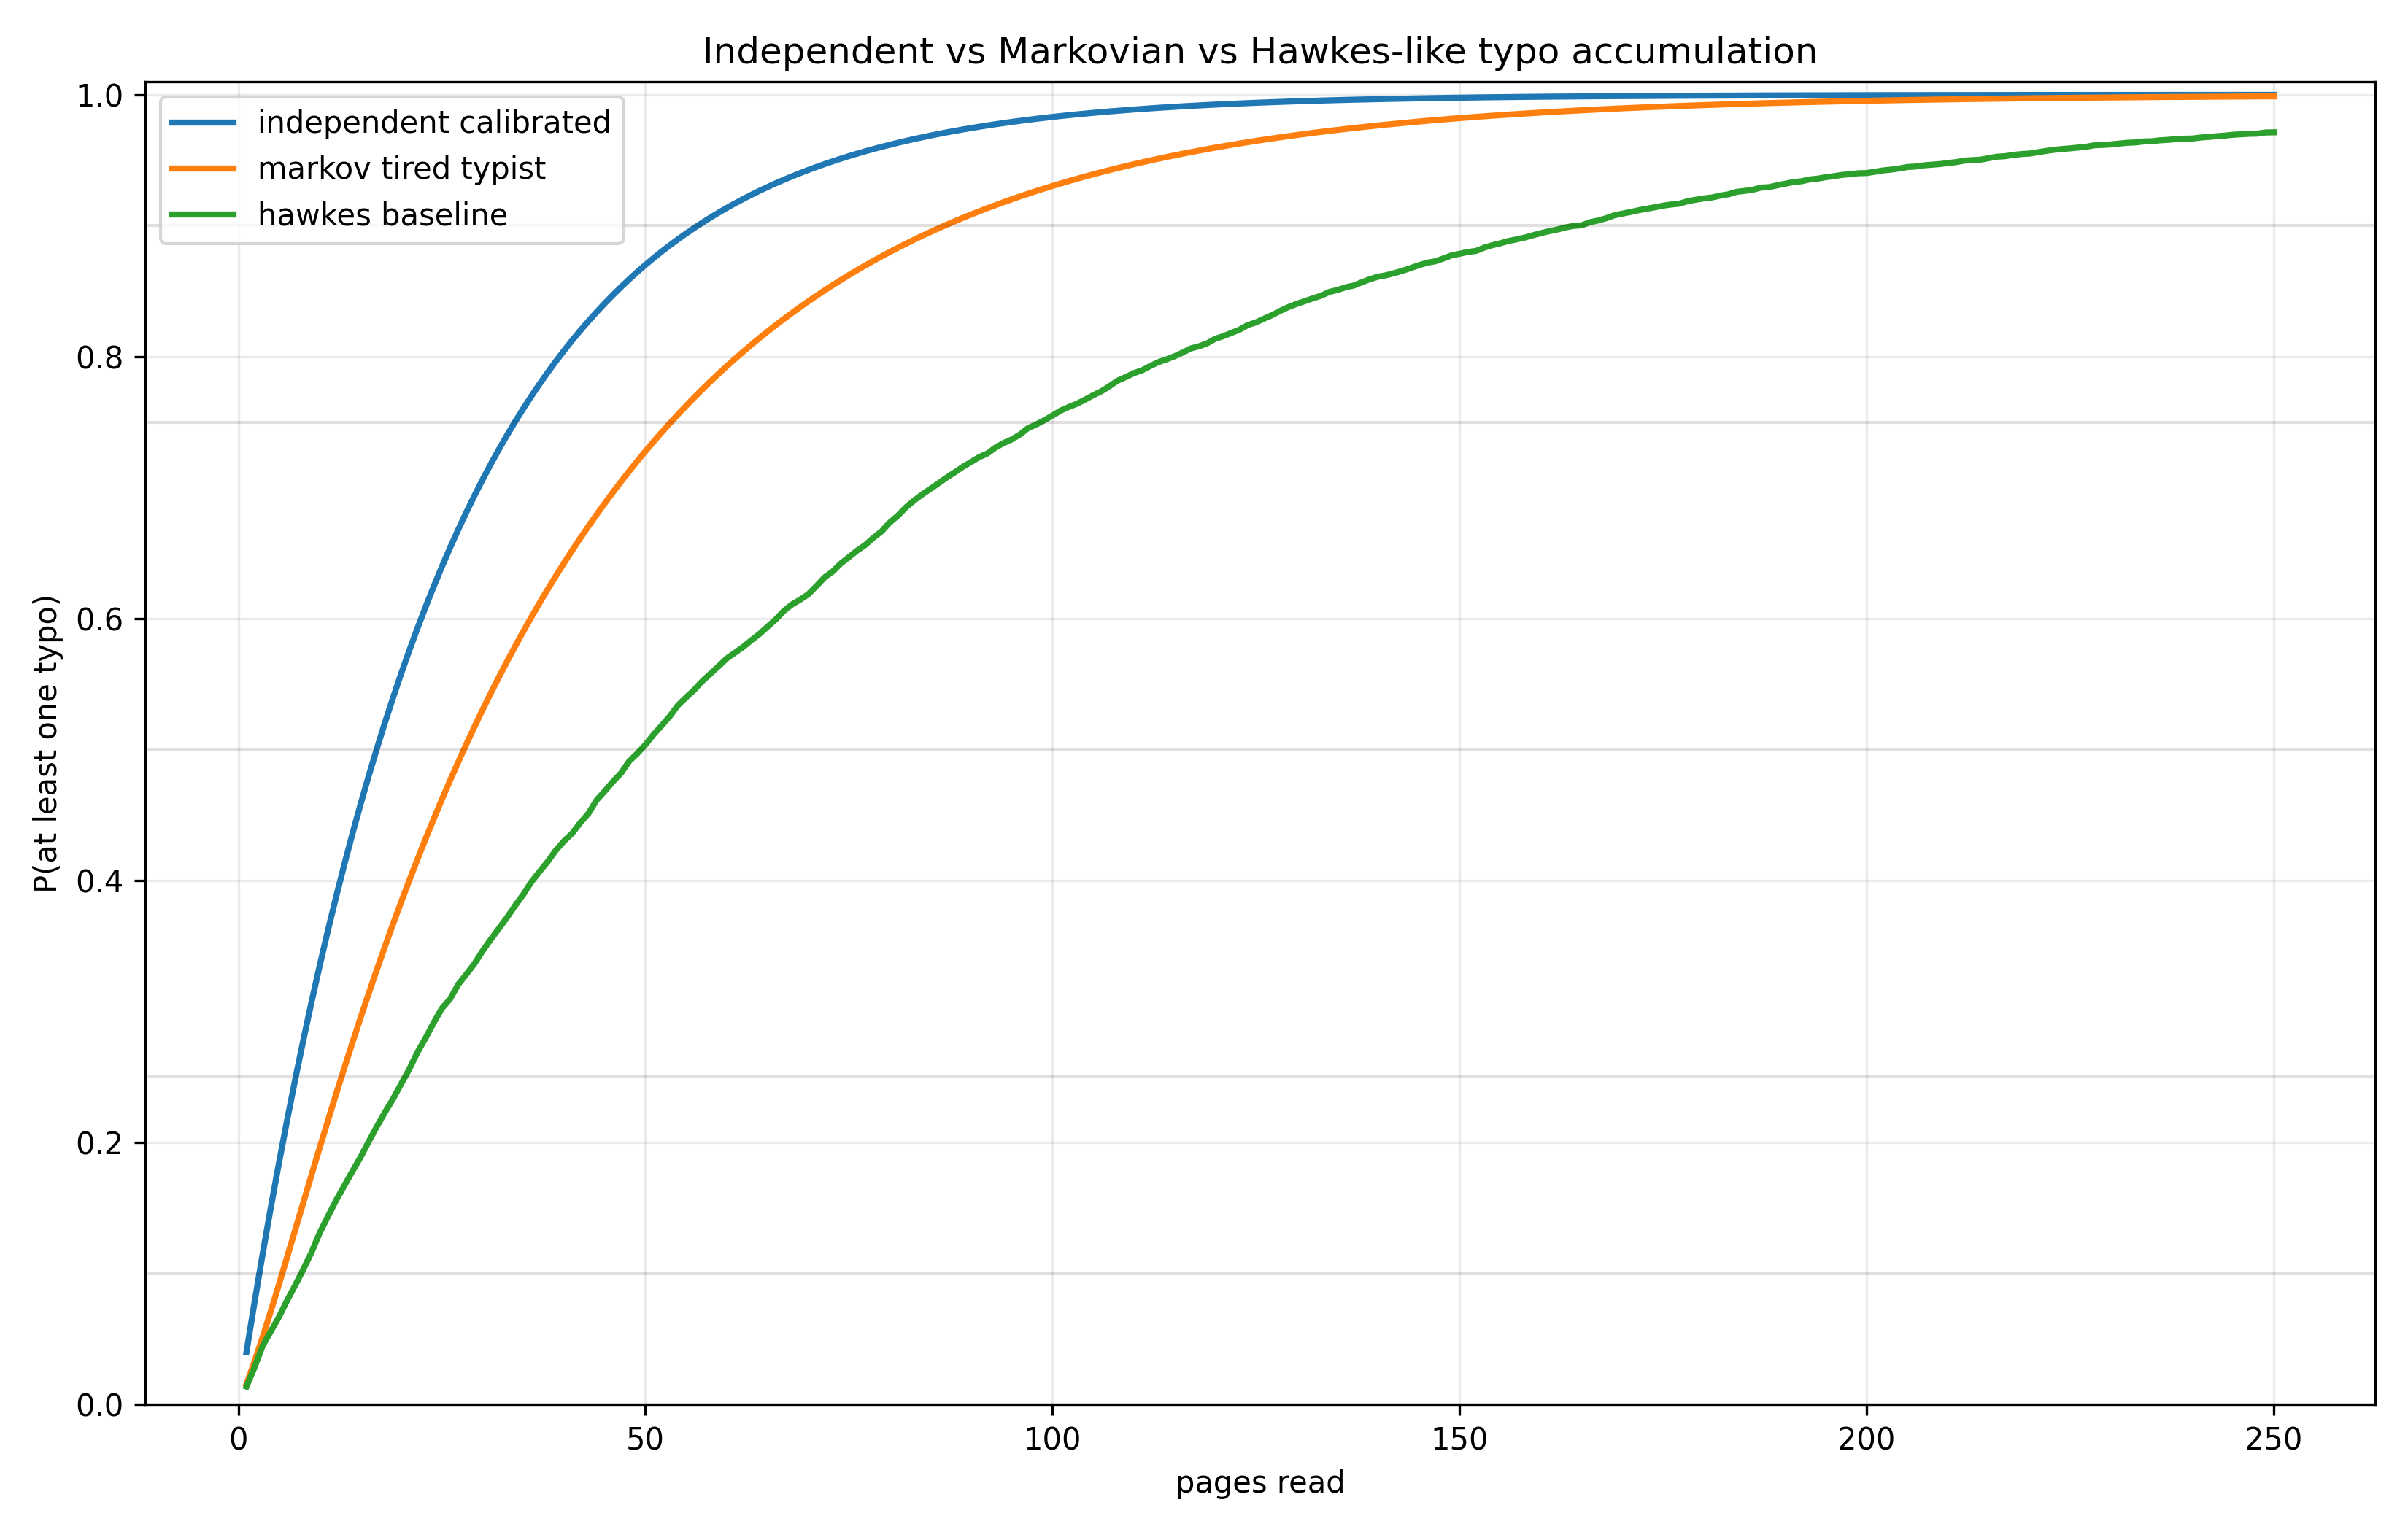
\includegraphics[width=0.92\linewidth]{hawkes_model_comparison_curves.png}
  \caption{Cumulative probability comparison. The calibrated independent model,
  hidden Markov model, and Hawkes-like model can differ substantially in first
  crossing behavior, but this plot alone does not isolate clustering.}
  \label{fig:model-comparison}
\end{figure}

\subsection{Inter-Typo Gaps}

The inter-typo gap distribution is the sharpest illustration of
self-excitation. In the independent model, gaps are roughly geometric. In the
hidden Markov model, short gaps become more common because tired stretches
persist. In the Hawkes-like model, a typo directly lifts the near-future
hazard, placing still more mass on gaps of one or two pages.

\begin{figure}[htbp]
  \centering
  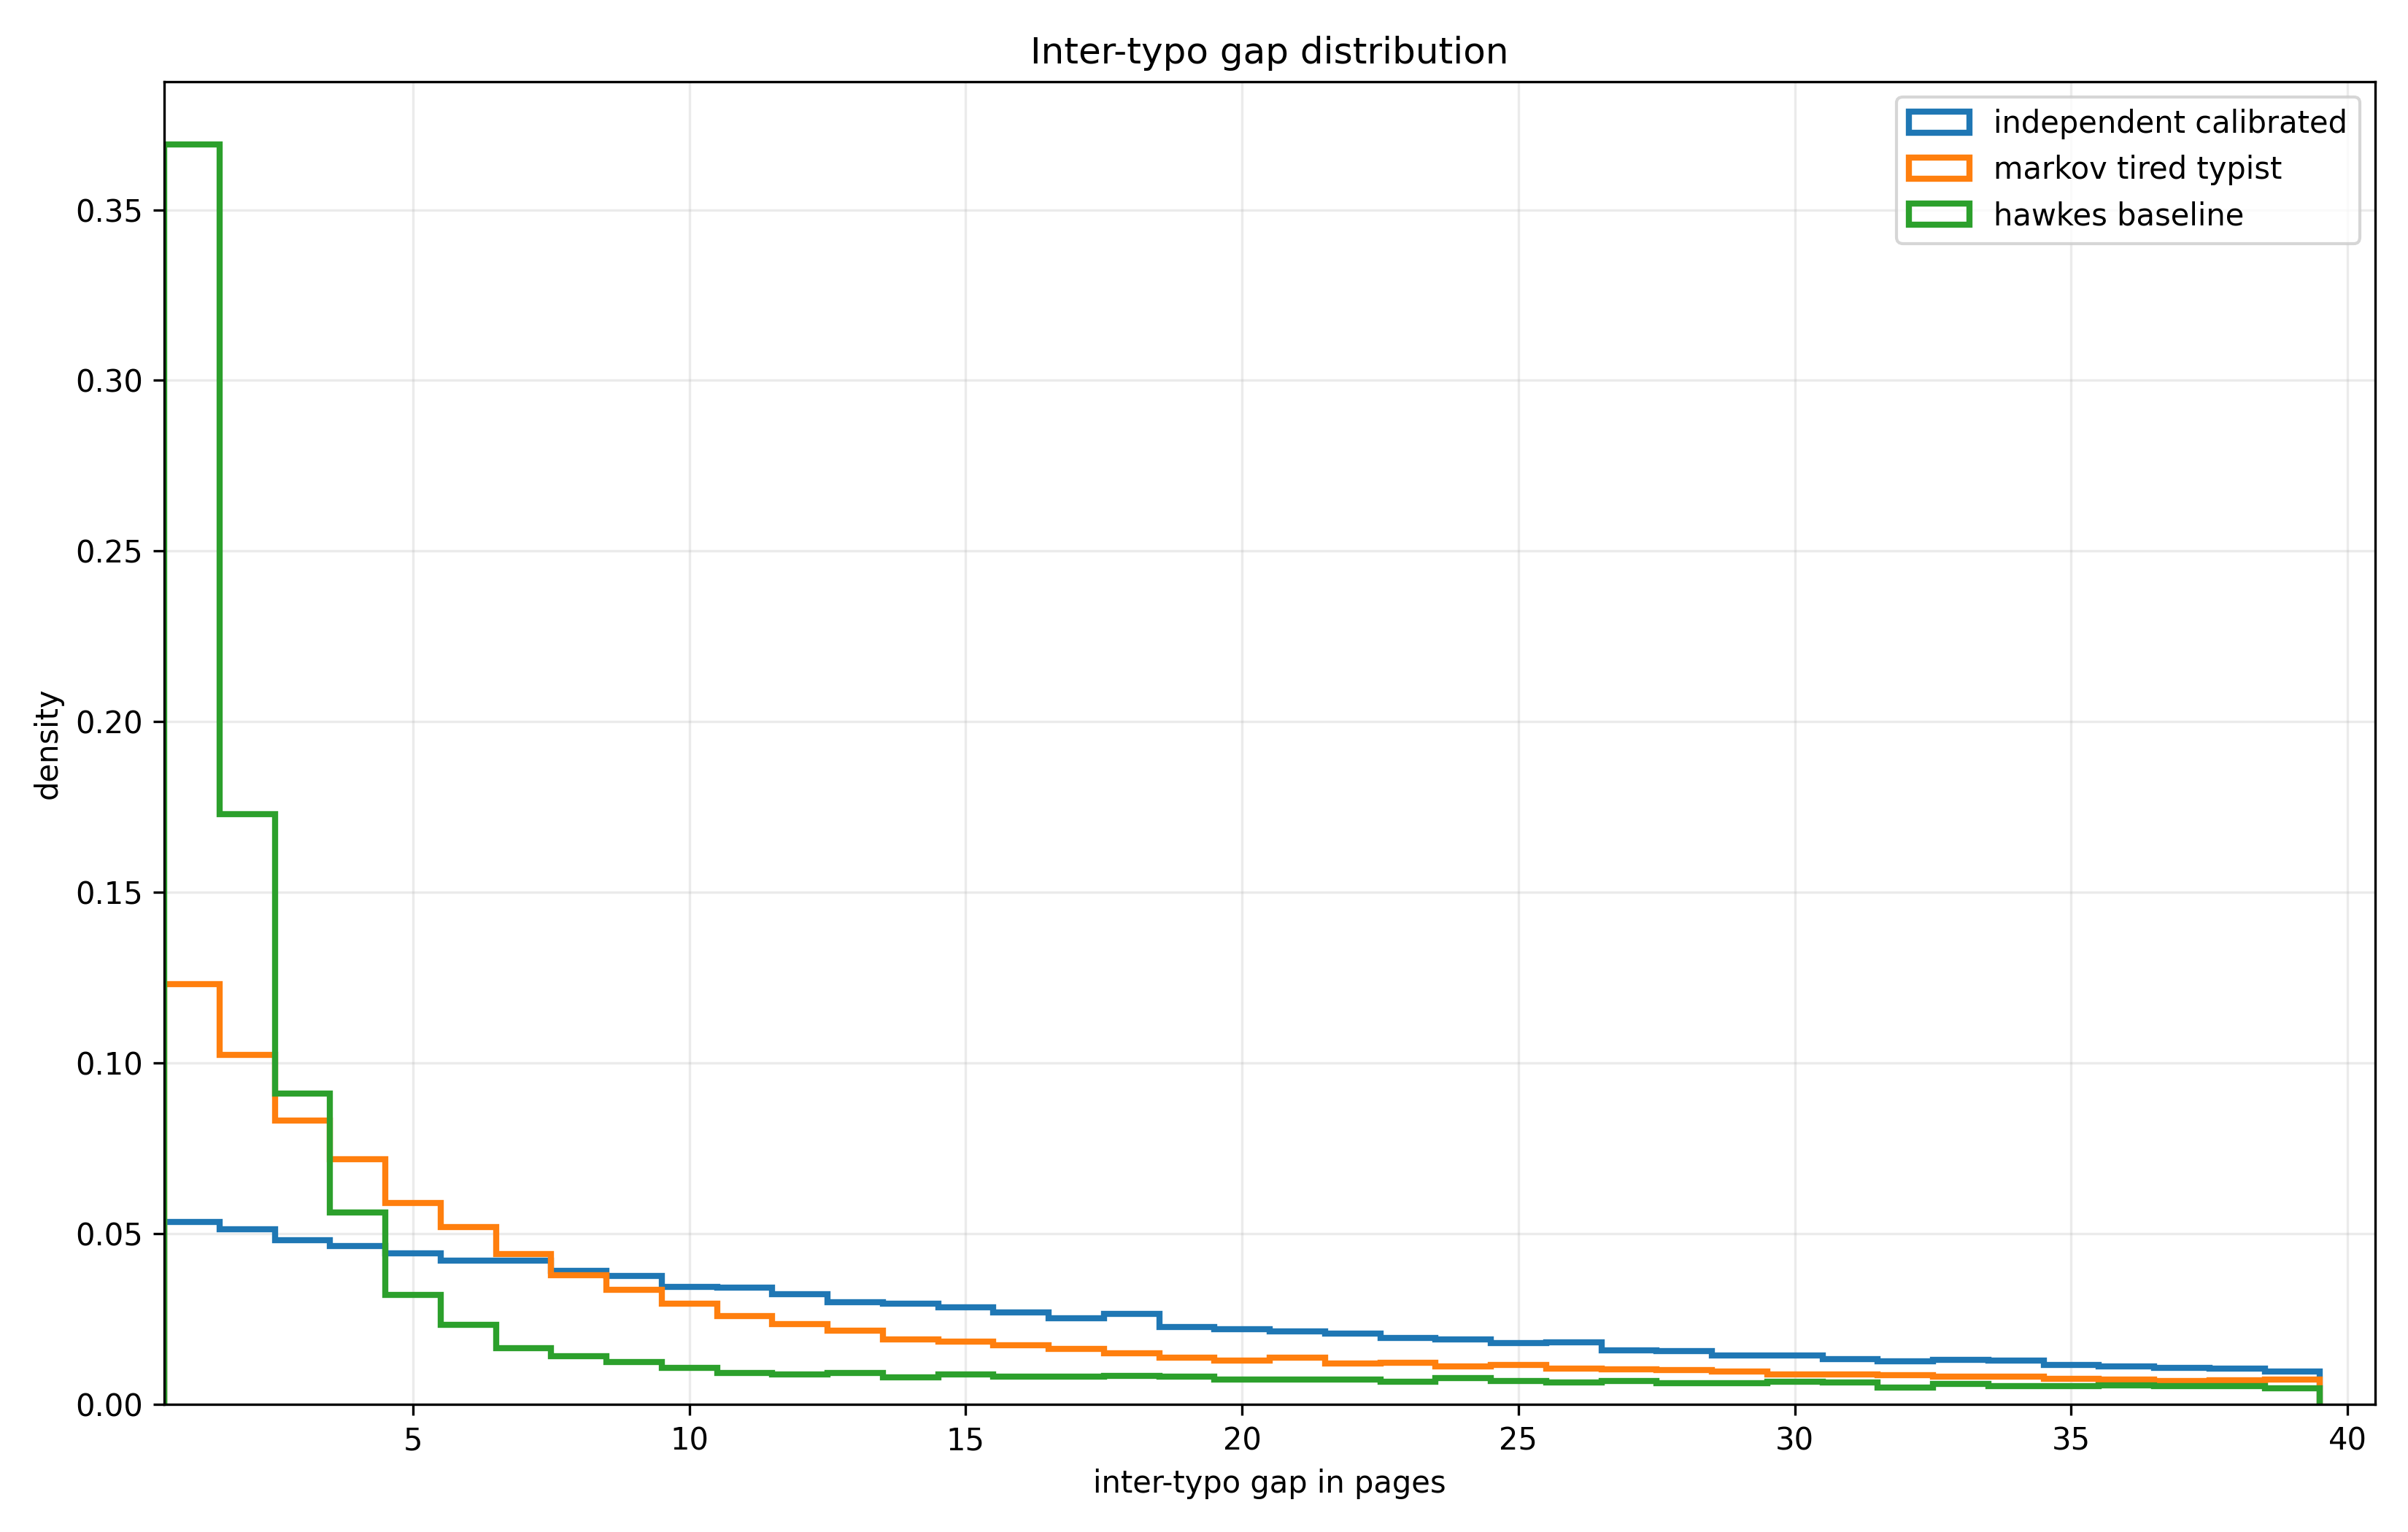
\includegraphics[width=0.92\linewidth]{hawkes_inter_typo_gap_comparison.png}
  \caption{Inter-typo gap distributions. This is the most revealing plot in
  the experiment: the Hawkes-like process puts much more mass on very short
  gaps, showing self-excitation directly.}
  \label{fig:gap-comparison}
\end{figure}

\subsection{Burst Sizes}

To summarize clusters, define a burst as a group of typos where consecutive
typo pages are at most two pages apart. The resulting burst size distribution
again separates isolated errors from self-excited clusters.

\begin{figure}[htbp]
  \centering
  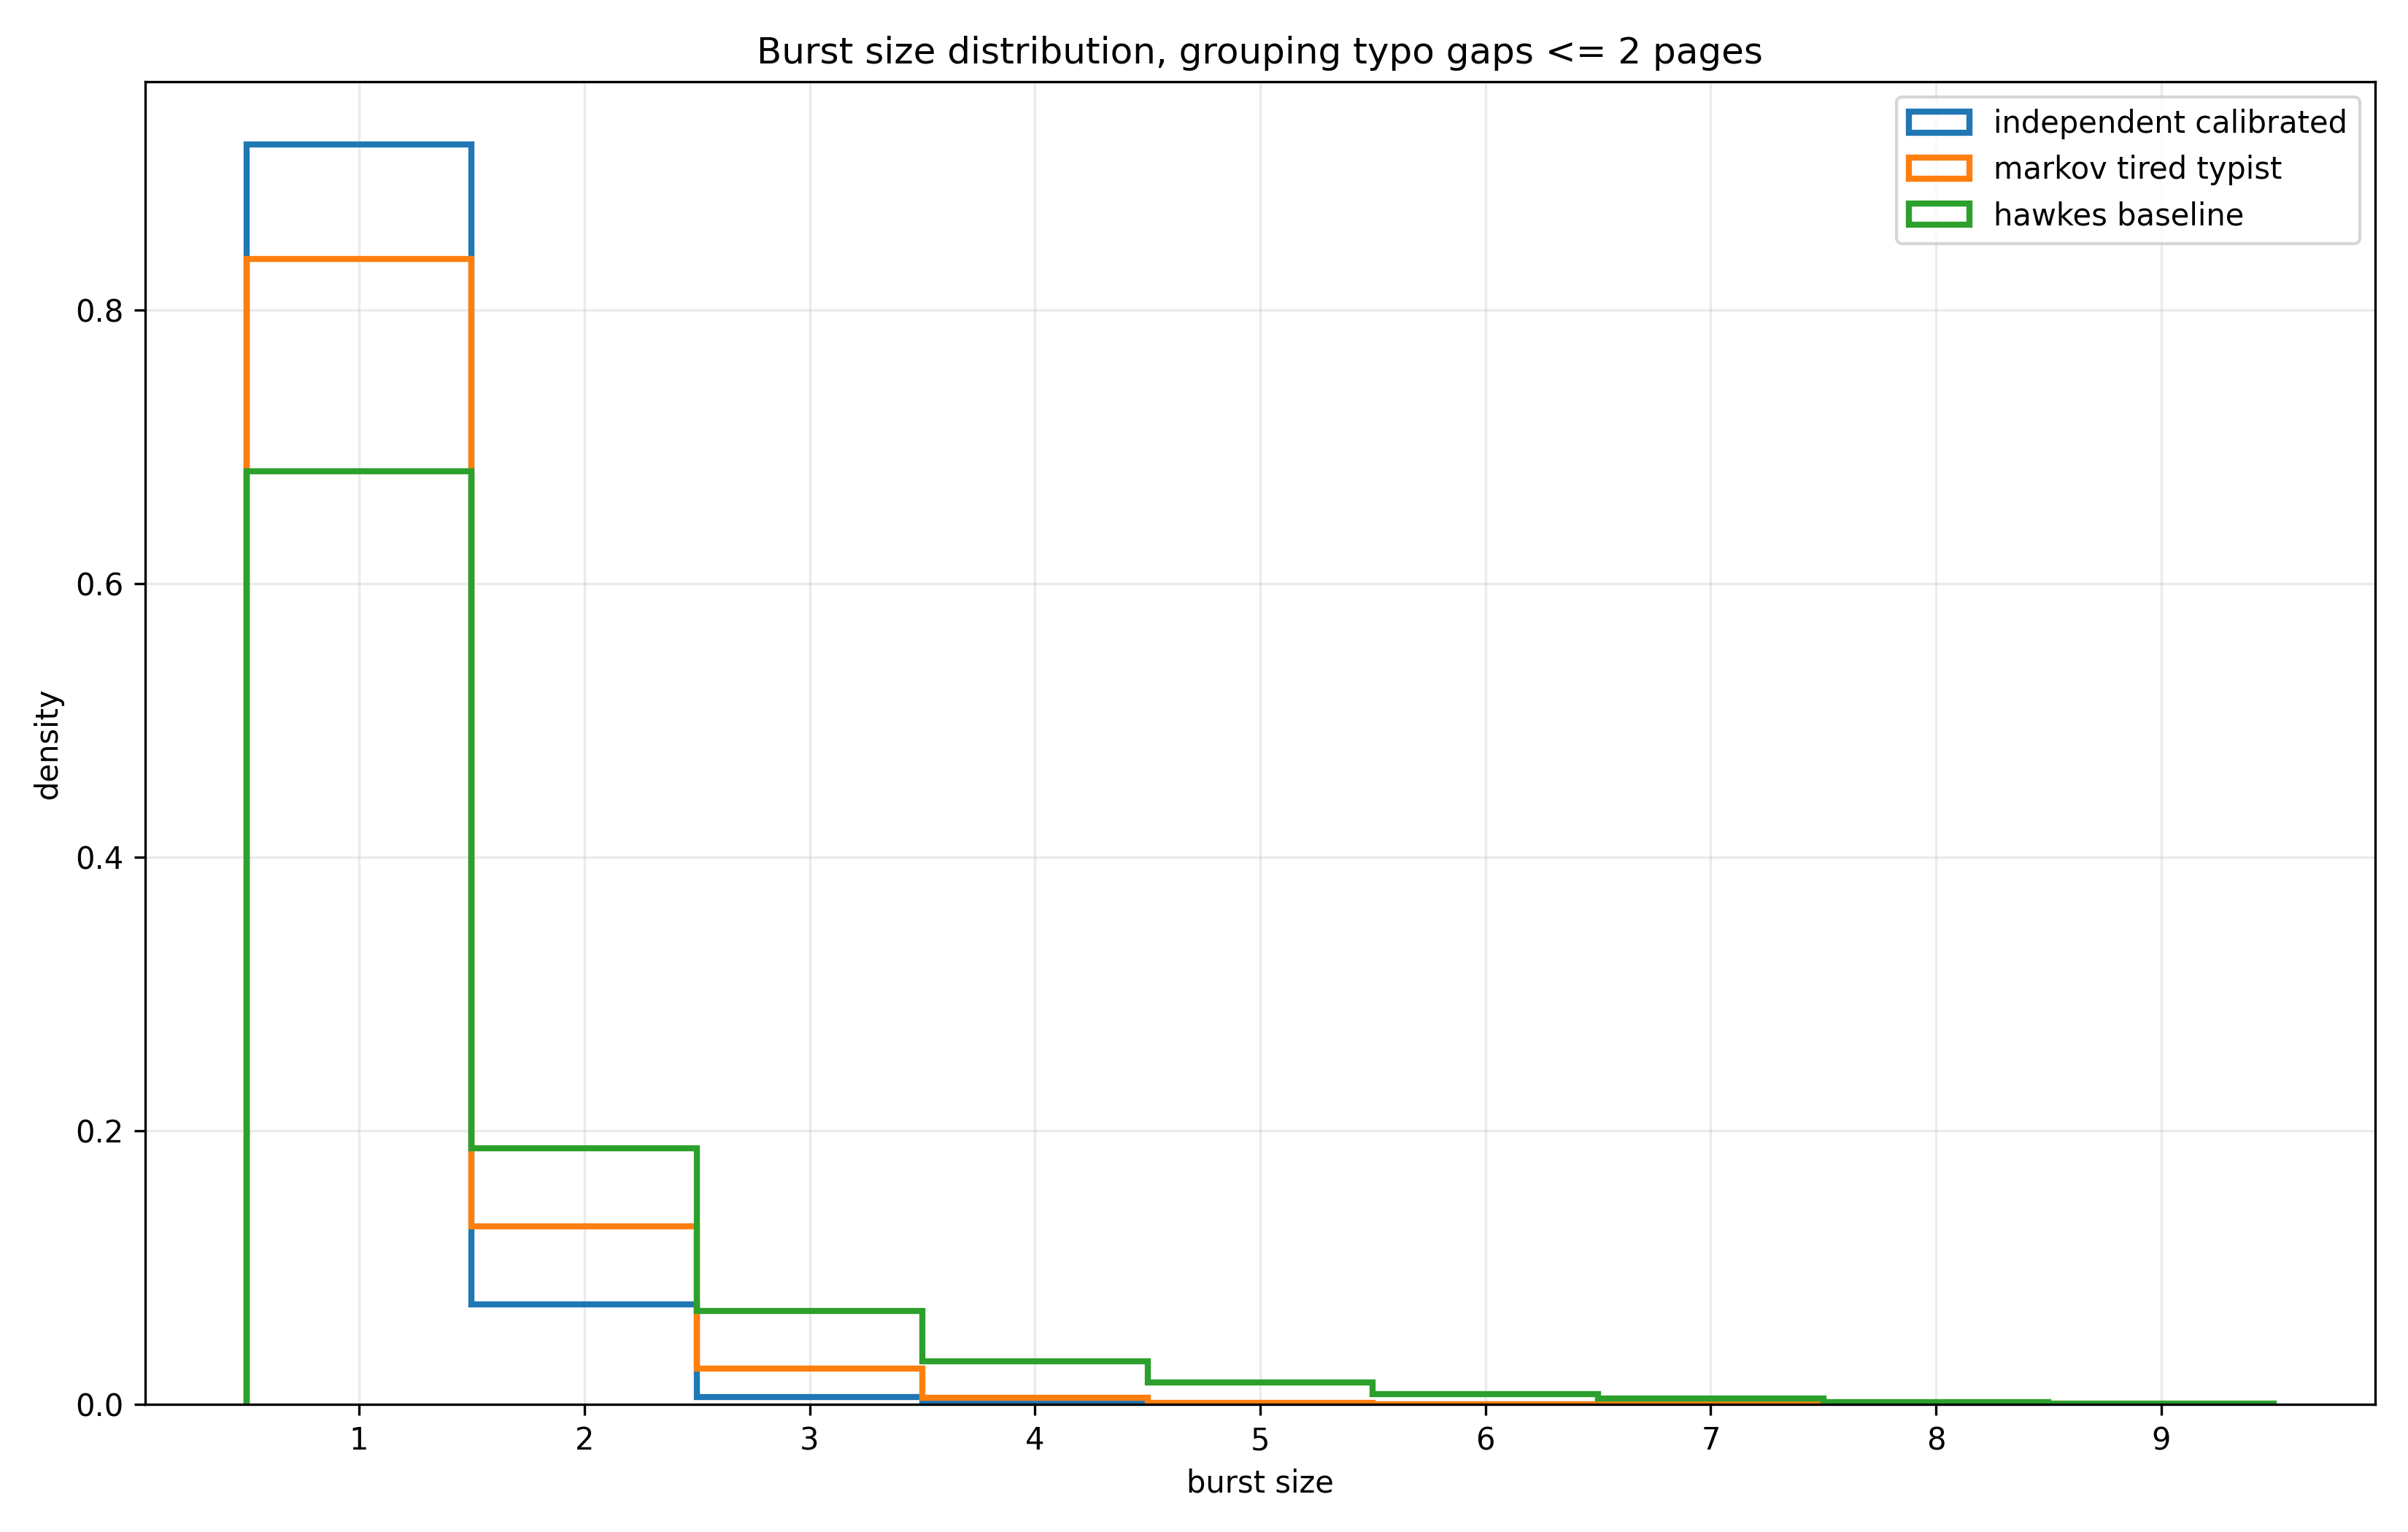
\includegraphics[width=0.92\linewidth]{hawkes_burst_size_comparison.png}
  \caption{Burst size distributions, grouping typo gaps of at most two pages.
  Self-excitation increases the frequency of multi-typo bursts.}
  \label{fig:burst-comparison}
\end{figure}

\section{Numerical Summary}

The default simulation used \(8000\) Monte Carlo paths of \(250\) pages for
the simulated comparisons. The most useful summary statistic is the probability
that an inter-typo gap is at most two pages:
\[
\Prb(\text{gap}\le 2).
\]
In the default run, this quantity is approximately
\[
\begin{array}{rcl}
\text{independent calibrated} &:& 0.09,\\
\text{hidden Markov tired typist} &:& 0.19,\\
\text{Hawkes baseline} &:& 0.43.
\end{array}
\]
Thus the Hawkes-like model has fewer total typos than the calibrated
independent and Markov baselines in this particular parameterization, but its
typos are far more clustered. This is exactly the qualitative signature the
point-process model was meant to expose.

\begin{figure}[htbp]
  \centering
  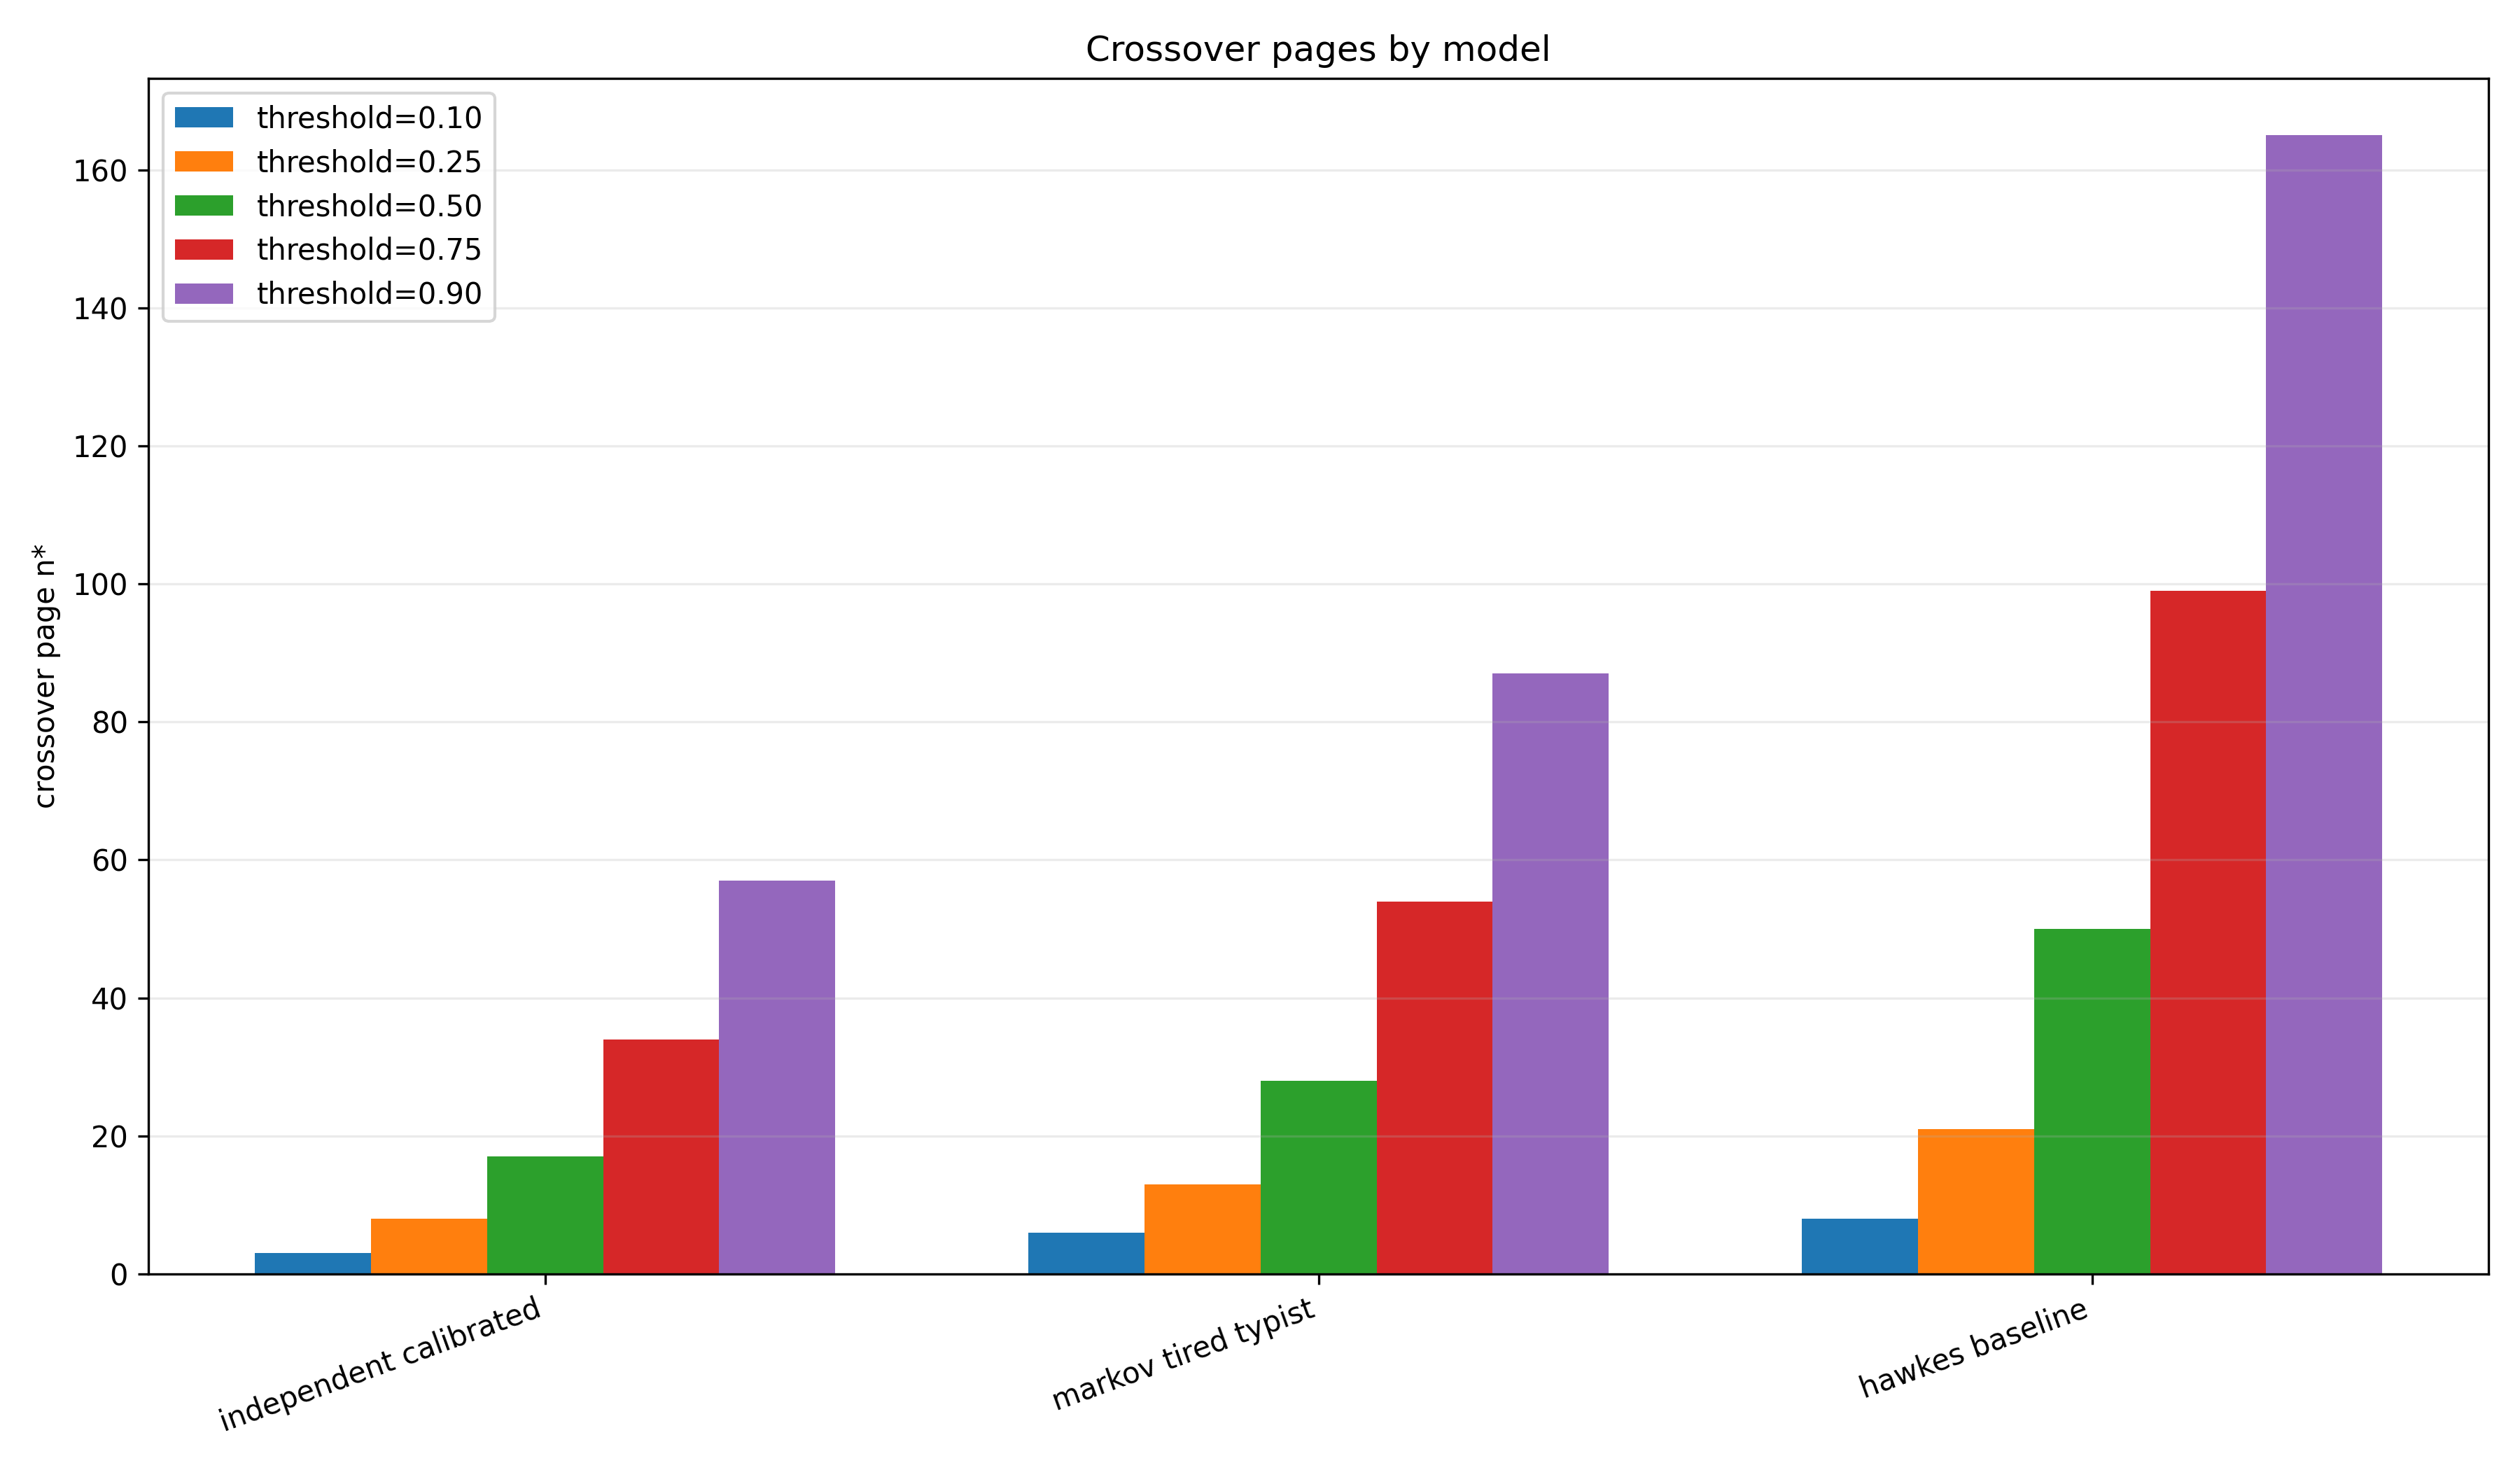
\includegraphics[width=0.92\linewidth]{hawkes_crossover_comparison.png}
  \caption{Crossover pages by threshold for the three comparison models. The
  Hawkes baseline is slower to produce the first typo in this parameterization,
  while still being more clustered conditional on typos appearing.}
  \label{fig:crossover-comparison}
\end{figure}

\section{Discussion}

The three models differ by where dependence enters.
\[
\begin{array}{lll}
\text{Independent model} &:& \text{no dependence between pages},\\
\text{Hidden Markov model} &:& \text{dependence through latent tiredness},\\
\text{Hawkes-like model} &:& \text{dependence through observed typo events}.
\end{array}
\]
The hidden Markov model says that typos are evidence of an unobserved state.
The Hawkes-like model says that typos themselves raise the immediate future
hazard. Both create bursts, but the inter-gap distribution shows that
self-excitation has a particularly direct signature: a heavy concentration of
very short gaps.

The lesson is modest but useful. Even in a toy typo problem, the modeling
choice determines whether errors look like isolated accidents, symptoms of a
persistent latent condition, or events that excite further events. The plots
make these mechanisms visible.

\end{document}
